\part{Materials and Methods}

The results of the present work come from the computational analysis of diverse Next generation sequence (NGS) experiments. These NGS experiments and the treatment of embryos were done by other people in the lab. Although how these experiments are done is out of the scope of this computational thesis, I would like to acknowledge the people that did them. In the first part of the project, the drug treatments and NGS experiments were done by Sandra Jimenez \parencite{magri_assaying_2020}. In the second part of the project, the ATAC-seq experiments in \textit{Astyanax mexicanus} were performed by Elisa de la Calle, in Woodshole.

The explanation of these analyses ought to be reproducible and clear for all the people reading this work. In order to achieve that, the scripts used for computational analysis had been deposited in \href{https://github.com/alexgilgal/Thesis_methods}{this GitHub repository}.


\chapter{Computational Analysis}

In this chapter, we will explain the computational methods that have been used to produce the Results. Since computational methods are constantly evolving, there have been several iterations in how the data was analyzed, and it may vary in some details from one project to the other. In order to address this problem, we have generated a GitHub repository in which the main analyses have been posted. During this chapter, we will refer to it several times. The steps of those pipelines will be explained in detail. 

In the next table, there is all the information about genomes and gene annotations used for mapping RNA-seq or ATAC-seq.

\begin{center}
\begin{tabular}{ |c|c|c| } 
 \hline
 Species & Genome Assembly & Source \\
 \hline
 \textit{Branchiostoma lanceolatum} & Bl71nmer & \href{http://amphiencode.github.io}{Amphiencode }\\ 
 \textit{Danio rerio} & danRer10 & \href{http://hgdownload.soe.ucsc.edu/goldenPath/danRer10/bigZips/}{UCSC} \\
 \textit{Astyanax mexicanus} &  (AstMex2) & \href{http://Feb2023.archive.ensembl.org/Astyanax_mexicanus/Info/Index}{ENSEMBL}\\
 \textit{Xenopus tropicalis} & xenTro10 & \href{http://hgdownload.soe.ucsc.edu/goldenPath/xenTro10/bigZips/}{UCSC}\\
 \textit{Ptychodera flava} & Pfla1 & \href{http://octopus.unit.oist.jp/HEMIDATA/pfl.genes.gff3.gz}{Hemidata}\\
 \hline
\end{tabular}
\end{center}

\section{ATACseq}

\subsection{From raw fastq files to data visualization}

We have used two sets of files, one for each chapter of the Results of this thesis. 
\begin{itemize}
    \item The first set of data corresponds with the analysis of amphioxus and zebrafish developmental pathways, and their pharmacological disruption. These experiments consist of samples proceeding from embryos treated at 30\% of epiboly until stage 80\% of epiboly. Embryos were treated with four different sets of pharmacological compounds which affect key developmental signalling pathways. Each treatment has two replicates of ATAC-seq. In total, we have eight samples per species.
    \item The second set of data corresponds with the study of gene regulation and its impact on the cave adaptation in \textit{Astyanax mexicanus}. In this case, we have four different developmental stages in both surfacefish and cavefish. These stages are 80\% epiboly, five somites (5ss), twenty-four post fertilization (24hpf) and forty-eight hours post-fertilization (48hpf). In total, we have eight samples per population.
\end{itemize}

We developed a pipeline in order to process in a consistent manner the ATAC-seq raw data. For both sets of data previously mentioned, this pipeline was used. This pipeline can be found in the GitHub repository in the folder ATAC-seq, under the name \path{ATAC_pipe.pl}. This pipeline consists of the next steps:
\begin{itemize}
    \item Mapping of reads: Reads were mapped against the reference genome using Bowtie2 \parencite{langmead_fast_2012}. The reference genomes used were danRer10 (zebrafish), Bl71 (amphioxus), and AstMex2. Reads pairs that had an insertion length larger than 2kb were filtered out. The result of this step produces a bam file with aligned reads.
    \item Filtering and centring of reads: Reads stored in the bam file are transferred to a temporal BED file. Those reads whose insert size was less than 130 bp were marked as nucleosome-free reads and were kept. The Tn5 cut position was established moving the start of the reads -4 bp in the reverse strand and +5 bp in the forward strand. This position was extended by 5 bp in both directions. This step resulted in a BED file with those positions.
    \item Transformation of BED to BigWig. The cut positions stored in the BED were extended to 100 bp. These extended reads were used by the wigToBigWig tool to transform the BED file into a BigWig file that could be loaded in any genome browser. In our case, it was the UCSC genome browser. 

\end{itemize}

The resulting files of the \path{ATAC_pipe.pl} were used for identifying open chromatin regions in the corresponding genomes. In our case, ATAC-seq peaks were identified using IDR \parencite{li_measuring_2011}. Briefly, this method allows us to account for biological replicates in a sequencing experiment and allows us to get the set of peaks that are consistent between our replicates. The resulting BED files from the previous pipeline are fed to the \path{idr_ATAC_script.sh}, which can be found in the GitHub repository. This script will generate several files, but the one that interests us the most is the one that contains the consensus peaks between replicates. Once we have this BED file, we will have one set of peaks for each of our conditions. These bed files can be uploaded to the browser in order to visualize the open chromatin regions in the corresponding genome.

\subsection{Differential analysis of ATAC-seq}

Differential analyses were carried out using the R package DESeq2 \parencite{love_moderated_2014}. Due to the requirements of this package, ATAC-seq data has to be preprocessed in order to compute these analyses. The preprocessing of this data consist of the following steps, performed with the bedtools suit \parencite{quinlan_bedtools_2010}. 
\begin{itemize}
    \item The first step consists of the aggregation of all the peaks of the samples that will be analyzed. We will merge all the IDR peaks of the different samples in a unique BED file, which will contain all the open chromatin regions across all samples. 
    \item The second step consists of the mapping of the ATAC-seq reads to this BED file, in order to get a quantification of how many reads are inside these peaks for each sample. This will produce a BED file for each of our samples (including replicates). All these BED files will have the same number of peaks.
    \item The third step formats the resulting BED files from the previous step in a DESeq2-friendly way. We need to keep only two columns for each sample, the peak ID and the quantification. With this final step, the resulting txt files have the same format as HTSeq files, which are readable directly by DESeq2.
\end{itemize}

Provided the unimodal quantitative nature of ATAC-seq data, we used DESeq2 to infer differentially accessible regions of open chromatin. An example of this is given in the GitHub repository (\path{ATAC_deseq2.R}). We have used a Benjamin-Hochberg $P value < 0.05 $ as a cutoff for the statistical significance of differential peaks. Using this script will provide the user with several results files. This script will write a table with the differential results in a table which contains all the statistical information extracted from DESeq2. Separately, there will be two BED files, which correspond to the genomic positions of the differential peaks, under and overexpressed. These files will be used in the following steps.

\subsection{Motif enrichment}
\label{meth:motif_enrichment}

Given a set of ATAC-seq peaks, we can compute which TFBS are enriched in that set of peaks. For this, we can estimate the probability of finding a given TFBS inside a specific set of genomic regions. This probability is compared to the probability of finding this motif in a background set of genomic regions, and then we can compute the enrichment of the TFBS in the specific set of regions. In the case of the differential peaks, we take the over and underexpressed set of peaks and compute the TFBS enrichment in both cases. This is done using the HOMER tool suit \parencite{heinz_simple_2010}. We used the findMotifGenomes.pl tool, providing as a genomic background the complete set of ATAC-seq peaks which we have tested for differential expression. We have taken into account for enrichment only vertebrate motifs. The GitHub repository contains a script that analyses the necessary inputs with fixed parameters in order to preserve reproducibility. This script can be found in the ATAC-seq folder under the name \path{homer_enrichment.sh}. The resulting plain text tables and HTML tables are used for interpreting results. In some cases, when we have combined the outputs of HOMER, we need the txt files to plot the combination in a dot plot. This dot plot is produced with the script \path{combine_Homer.R}. In the end, this script produces a dot plot in which the X axis are the samples and the Y axis are different motifs. The dot size represents the enrichment score and the colour of the significance of that enrichment.

\subsection{Assigning of target genes to each ATAC-seq peak}

Peak gene association is one of the most critical steps after ATAC-seq data analysis. This is not a trivial task, but one extended practice in the field is to assign the closest genes to the peaks. We keep two genes upstream of a peak and another two downstream of it. We then filter out those assigned genes more than 1 Mb away from the ATAC-seq peak. The reason to keep genes upstream and downstream is to avoid leaving unassigned genes for each of the peaks. 

We also used GREAT \parencite{mclean_great_2010} as an alternative method for assigning genes to peaks. Briefly, the GREAT method assigns a fixed region around the TSS of a gene, in which whatever peak that falls within, will be assigned to that gene. These regions are known as basal regions. Afterwards, an extended region is computed for each gene, in which the basal region is extended until it reaches 1 Mb or overlaps with another basal region of another gene. Basal regions can overlap between them, but an extended region can not overlap with the basal region of another gene. 

The results of both methodologies, GREAT and closest gene, are overlapping, and the choice of one over the other do not alter the results in a significant way. 

As a result of both methods, we obtain a list of genes assigned to peaks. This will output will be used for integrating ATAC-seq and RNA-seq, which is discussed in detail in the section \ref{sec:integration_atac_rna}. Furthermore, the resulting gene list can be analyzed. In our case, we have computed Gene Ontology enrichment analysis. How we did it is discussed in the next section, in \ref{sec:RNAseq}.

\subsection{Clustering of ATAC-seq signal}

In both chapters of the results, we have used ATAC-seq signal clustering as a powerful tool to see differences between our samples. These clusterings were produced using Deeptools \parencite{ramirez_deeptools2_2016} and seqminer \parencite{ye_seqminer_2011} software. The computation of the cluster was done in seqminer, where we provide the BigWigs files. This software uses k-means clustering, a supervised clustering algorithm that needs the user to establish the number of clusters that will be computed beforehand. We used 12 clusters, but we kept the most representatives. The resulting clustering was then exported to a BED file which contained the positions for each cluster of peaks. This BED file was then fed to deeptools in order to generate the visualization of these clusters.


\subsection{Discovering mutations that disrupt TFBS in ATAC-seq data}

We used CRISP software \parencite{bansal_statistical_2010} in order to obtain the ATAC-seq regions that have mutations. CRISP is a software whose main function is to call variants from NGS data. The script used in order to produce this analysis was deposited in the GitHub repository. This program needs as input the following files:

\begin{enumerate}
    \item The aligned reads of ATAC-seq samples in BAM file. These BAM files were processed by the $MarkDuplicates$ tool from the Picard toolset. The parameters for this processing step are in the script deposited in GitHub.
    \item The reference genome to which the samples were mapped. In our case, this was the AstMex2 genome (surfacefish genome).
    \item The set of genomic regions the user wants to interrogate in BED format. In our case, this was all the ATAC-seq regions detected across all ATAC-seq samples.
    \item A TXT file that indicates to what sample corresponds to each BAM file. The TXT file used for our analysis has been deposited in GitHub.
\end{enumerate}

The output of CRISP was a VCF file which contained the variations detected. This VCF file was filtered in order to keep only those variants that were specific to cavefish. The script used for this filtering is deposited in GitHub. The filtered VCF was intersected with ATAC-seq peaks using $bedtools intersect$. 

In order to know if these mutations affected TFBS inside ATAC-seq peaks, we used the R package MotifBreakr \parencite{coetzee_motifbreakr_2015}. This package takes as input a VCF file, the genome in 2bit format, and a database of motifs scores. In our case, we provided the filtered VCF file, the AstMex2 genome in 2bit format and the entire JASPAR vertebrate motifs database \parencite{castro-mondragon_jaspar_2022}. The result was a table which indicated to which extent a mutation was altering the motif score in the mutated vs the reference genome

Finally, to test that the TFBS impairment was affecting the binding of TFs, we used TOBIAS \parencite{bentsen_atac-seq_2020}. This tool detects if a given TF is binding to the genome by using the fingerprint of the binding of each TF. These are the inputs that TOBIAS needs:
\begin{enumerate}
    \item A motif collection. We used the same than for MotifBreakr.
    \item The ATAC-seq BAM files. We used all our ATAC-seq samples, dividing them in cavefish and surfacefish.
    \item A genome and annotation. We used the AstMex2 genome in FASTA format and its corresponding annotation from ENSEMBL in GTF format.
\end{enumerate}

TOBIAS uses a snakemake pipeline in order to make the results reproducible. This pipeline requires the user to put the parameters of the analysis in a $config.yaml$ file. The $config.yaml$ used in our analysis is available in GitHub.

The pipeline of TOBIAS generated several folders of results. One of these outputs was how each TF is binding to the genome and if there are differences between cavefish and surfacefish in how these TF binds to the genome. We crossed this information with the results of MotifBreaker to produce the Figure \ref{fig:Motifbreakr_tobias}. This crossing of information is documented in a script in the GitHub repository.


\section{RNAseq}
\label{sec:RNAseq}

\subsection{From raw data to data visualization}

RNA-seq was used to assess the transcriptomic output of epigenetics. Just like with ATAC-seq, we have used two sets of samples for our analyses.
\begin{itemize}
    \item The first group of samples correspond to the first chapter of the results (\ref{sec:Interconnectivity_chapter}). We have the equivalent samples for Amphioxus and zebrafish as in the previous section. These experiments consist of samples proceeding from embryos treated at 30\% of epiboly until stage 80\% of epiboly. The embryos were treated with four different sets of pharmacological compounds which affect key developmental signalling pathways. We have three replicates of RNA-seq per condition. For zebrafish and amphioxus, this translates to a total of 15 fastq files (5 conditions including control with 3 replicates each of them). We also have transcriptomic information for \textit{Xenopus tropicalis} and \textit{Ptychodera flava}. In the case of these two species we only have data for two of the treatments, Nodal and FGF inhibitors. In these species, we have a total of 9 fastq files per species.
    \item The second set of samples corresponds to the second chapter of results (\ref{sec:cap_astyanax}). In this case, we used publicly available samples from the SRA archive with id PRJNA258661. This dataset consists of samples of \textit{Astyanax mexicanus} taken from embryos at different developmental points. These developmental stages are 10 hpf, 24hpf, 36 hpf and 72 hpf. There are 3 replicates by developmental stage and samples were taken from both surfacefish and cavefish (Pachón morph). 

\end{itemize}

The first step in our analysis is to assess the quality of the samples. This is done using the FastQC tool, which allows comprehensive yet easy quality control of our samples. 

Once every sample has passed QC we proceed to the mapping of the raw reads stored in the fastq files. This uses STAR aligner (version 2.5.3) \parencite{dobin_star_2013}. The reference genomes were Bl71 and danRer10 for amphioxus and zebrafish, respectively. The result of this step is a BAM file containing the mapped reads. In order to quantify the amount of reads that each gene had we have used HTseq \parencite{anders_htseq-python_2015}. For \textit{Xenopus tropicalis} and \textit{Ptychodera flava} raw samples were directly pseudo-mapped with the reference annotations of the corresponding species with Kallisto \parencite{bray_near-optimal_2016}, with default parameters. 

BAM files were transformed to BigWig using the tool bamCoverage from Deeptools. These BigWigs can be loaded into genome browsers like the UCSC genome browser.

\subsection{Differential analysis of RNA-seq}

In the case of RNA-seq, the differential analysis is more straightforward than in ATAC-seq. The quantification files produced by either Kallisto or Htseq can be loaded directly in DESeq2 for differential gene expression analysis. There is an example of this step in the GitHub repository in the RNA-seq section, \path{deseq_rnaseq.R}. In this script, we set as statistical cutoff a corrected $P value < 0.05$ and also an absolute $log_2(FC) > 1$. These parameters are a good compromise between eliminating false positive genes and keeping biological differences. 

The results of this analysis are several files containing statistical information on the differential gene expression and a list of genes that are differentially expressed between conditions. These gene lists are the ones that can be integrated with those produced in the analysis of ATAC-seq. 

In the case of amphioxus, differentially expressed genes were also translated into zebrafish genes via orthogroups. We used orthogroups as a translation layer between amphioxus and zebrafish genes. This is because we do not have a functional annotation of genes, and we want to know the orthology relationship between Amphioxus responding genes and zebrafish responding genes. In the GitHub repository, the code for obtaining this relationship can be found in \path{Amphi_zebra_fams.R}. The input of this function are the  gene IDs of amphioxus and a table containing the orthology information between amphioxus and zebrafish genes. This table of orthology contains orthogroups, or gene families, to which each amphioxus and zebrafish gene belongs. For each amphioxus gene, the function identifies to which orthogroup this amphioxus gene belongs and retrieves the entire group of zebrafish genes that belong to the same orthogroup. Since zebrafish have undergone three rounds of WGDs, one amphioxus gene can have several zebrafish orthologs. This zebrafish gene list can be further analyzed, either in order to analyse similar responses between orthologs as in Figure \ref{fig:common_affected_genes} or to compute the enriched GO terms of this set of genes.

\subsection{GO enrichment analysis}
\label{sec:GO_enrichment}

Gene Ontology (GO) analysis is a method for annotating and comparing the functions of genes based on their biological roles. It involves mapping genes to a standardized vocabulary of biological terms and concepts, known as Gene Ontology. The GO terms are organized in a hierarchical structure, allowing for a comprehensive representation of gene function at various levels of biological organization. We can compute how a certain GO term is enriched in a gene dataset. To do that, we need to select the gene universe of the analysis. In our case, these were all the genes of the organism. Next, we must provide the GO algorithm with the gene set of interest. GO enrichment is then computed by a hypergeometric test, which will compute the probability that the GO terms of the set of genes are enriched compared to the gene universe. 

In our case, these analyses were pivotal for developing both results chapters. In the GitHub repository, the script \path{GO_enrichment.R} has the necessary code for performing these analyses. These analyses were carried out using the R package TopGO. Among the several algorithms that this package provides, we used the \path{elim} algorithm. This algorithm allowed us to take into account the hierarchical structure of GO terms, selecting only the most specific ones. We selected those GO terms that accomplished a $P value < 0.05$. Take into account that P value correction is not desirable, nor doable for GO terms, since the observations are not independent (because of the hierarchy in GO structure). 

The enriched list of GO terms can be used by several different tools in order to visualize these results. One of these tools is Revigo \parencite{supek_revigo_2011}, which allows visualizing GO enrichment results as dot plots. These plots have semantical axes, meaning that the representation will cluster together GO terms that are similar.
Another way of representing these results is using a dot plot similar to the one used in motif enrichment. A script that produces these kinds of dot plots can be found in the GitHub repository (\path{dotplot_GO.R}).

Furthermore, using the GOSemSim R package, we were able to compute similarities scores between sets of GO enrichments, which gives insight into how similar are two different lists of GO terms. An example of this is represented in Figure \ref{fig:ATAC_go_similar}.

\section{Integration of ATAC-seq and RNA-seq}

\label{sec:integration_atac_rna}

We used different methods in order to integrate the epigenetic and transcriptomic information. We will describe here these methodologies for this integration and where they have been used. We will first treat the simpler approach, and then we will explain the more sophisticated one. We will also explain here how we computed connectivity scores that have led to the results of the chapter \ref{sec:Interconnectivity_chapter}.

\subsection{Integration using gene lists}

As we mentioned in the previous sections, when analyzing ATAC-seq and RNA-seq separately, we generated gene lists. In the case of RNA-seq, those lists represent the genes that are differentially expressed between conditions. On the other hand, in the case of ATAC-seq, these lists represent the genes that are close to Differentially Accessible Regions (DARs). We integrated these two sets of genes by simply computing the intersection of both lists. The result was a list of genes that are differentially expressed and also have nearby a DAR. As shown in \ref{sec:Interconnectivity_chapter}, these genes were directly changing from one condition to another, and we called them Double Selected Genes (DSGs). 

Once we obtained these gene lists, we proceeded to perform different analyses like GO enrichment, thoroughly described in \ref{sec:GO_enrichment}. We also traced back which DARs are nearby these genes in order to obtain the set of peaks that were responsible for the epigenetic response of these DSG.

\subsubsection{Computing connectivity scores for ATAC-seq and RNA-seq}

Once we integrated a gene list of genes that respond at both epigenetic and transcriptomic levels, we computed the connectivity score of the aforementioned DSGs for the first chapter of the results.

The computation of this score is a simple yet powerful tool to understand how the different DGSs are connected to the altered signaling pathways in that part of the results. Once we had the gene list of DSGs that came from each of the treatments, we counted how many treatments each of the DSGs were responding to. This connectivity score goes from one (at least the gene is responding to one treatment), up to four (the maximum possible since we have four treatments). This connectivity score was computed not only for DSGs, and can actually be computed for a given condition if we have the gene list. It was computed even with ATAC-seq regions since the genomic position can be interpreted as geneID. In definitive, we have generated a powerful tool to compute how many times a gene or genomic location is responding to different treatments. This connectivity score can be then combined with other sets of genetic information, like how many copies have been retained for each gene (Figure \ref{fig:Connectivity_genes_wgd}), or how ancient the regulatory regions are (Figure \ref{fig:DARs_connect_evolutionary_age}).


\subsection{Integration using ANANSE}

There have been several attempts to integrate the ATAC-seq signal and RNA-seq signal in order to compute GRN. The main idea behind these attempts is to know which transcription factors are binding near genes that are changing their expression, using the DNA sequence of the nearby enhancers, TFBS and ATAC-seq signal. With this idea in mind, we can build GRN of TFs affecting genes, some of which can be TFs themselves.

Under this premise, ANANSE is born \parencite{xu_ananse_2021}. We used ANANSE to understand the GRNs that are driving the cave adaptation in \textit{Astyanax mexicanus} (see \ref{sec:cap_astyanax} for details). There is a PDF guide in the GitHub repository. This guide intends to recreate our analysis of \textit{Astyanax mexicanus} in a user-friendly manner.

As input, ANANSE needs several files. It needs the ATAC-seq data in BAM format, the quantification of RNA-seq normalized by TMP (which is obtained from Kallisto), the differential analysis of gene expression, and finally, a database of the TFBS. We have followed the next steps in order to integrate ATAC-seq and RNA-seq. There are explained in much more detail in the publication of ANANSE and in the documentation of the program that can be found in \path{https://anansepy.readthedocs.io}.

\begin{enumerate}
\item \textbf{Motif database orthology.} The first step is to accommodate the TF database that ANANSE has integrated. This database has been made for human and mouse genomes, and in our case, we have used it with \textit{Astyanax mexicanus}. ANANSE developers already thought of the possibility of running ANANSE for other species, and they provided a straightforward manner to transform the database from human and mouse to our species of interest using orthology inference. The tool $motif2factors$ allows us to transform the database. We ran this tool in order to translate the database to our \textit{Astyanax mexicanus} reference genome: AstMex2.
\item \textbf{Binding.} The second step computes binding scores for each TF in the open chromatin regions. This step integrates the previously transformed database with the ATAC-seq signal. Optionally in this step, we can give ANANSE the set of regions to be examined to TF binding. If not provided, ANANSE will identify peaks from the ATAC-seq BAM file, and it will use those peaks as regions of interest. As a result of this step, we obtain an h5 file which contains the computed binding score of each TF to all the interrogated regions. In our case, we used the IDR set of peaks as regions of interest for the 24hpf ATAC-seq of both surfacefish and cavefish.
\item \textbf{Network.} The third step needs as input the binding scores resulting from the previous step and the gene expression information in TPM. This step integrates the binding information with gene expression, and thus, here is where RNA-seq and ATAC-seq information is actually integrated. In this step, ANANSE computes an interaction score between TFs and target genes. This interaction score integrates the binding score of the TF, the distance of the enhancer to the target gene, the gene expression of the TF and the expression of the target gene. As a result of this step, we obtain an interaction list, which is ordered by the interaction score.
\item \textbf{Influence.} The fourth and final step is computing influence scores.  In this step, ANANSE can compare two different conditions (networks computed before). When comparing the networks of two conditions, ANANSE is able to extract which TFs are driving the transformation of the "source" network to the "target" network. In our case, we have used it to infer the GRN that drives the adaptation to the cave environment in cavefishes. The result of this step is a list of TFs and their influence score, which measures how important the TFs are for moving from one condition to another.
\end{enumerate}

\subsubsection{Using $seq2science$ in order to automatize preprocessing of data}

We want to address that a great amount of analysis can be automatised for all the samples that we have used. In fact, the last analysis done with ANANSE used data preprocessed by pipelines, like the aforementioned seq2science. There are several pipelines, but we find this one especially interesting because of genome management. This pipeline allows for custom installation of genomes from different sources like Ensembl, UCSC and NCBI, along with gene annotations, using the $genomepy$ tool.

In our case, we have installed the AstMex2 genome using $genomepy$ and preprocessed the ATAC-seq and RNA-seq data using the pipelines available in seq2science. This allowed us to easily obtain the necessary inputs for ANANSE, like the motif database, gene expression in TPM, ATAC-seq bams and differential gene expression. The parameters and options for the pipeline were the default for both analyses. The results from these pipelines are deposited in GitHub.

\section{Comparative genomics}
\label{sec:comp_genomics}
For our evolutionary analyses, it has been key to use comparative genomics and genome alignments as tools. Here we will describe how we have used different tools in order to obtain evolutionary insights from epigenomic and transcriptomic data.

\subsection{Genomics aligments}

The generation of genomics alignments was done using Progressive Cactus \parencite{armstrong_progressive_2020}. Progressive Cactus is a reference-free genome aligner, which has allowed researchers to align hundreds of vertebrate genomes efficiently. We used this program in order to align several teleost fish genomes, including both morphotypes of \textit{Astyanax mexicanus}. We included the next species in our genomic alignment of teleost fishes: \textit{Astyanax mexicanus} both morphotypes, \textit{Danio rerio} (zebrafish), \textit{Clupea harengus} (Atlantic herring), \textit{Oryzias latipes} (medaka), \textit{Esox lucius} (Northern pike), \textit{Pygocentrus nattereri} (red-bellied piranha), \textit{Pangasianodon hypophthalmus} (striped catfish), \textit{Electrophorus electricus} (electric eel), \textit{Sinocyclocheilus grahami} (golden line barbel), \textit{Ictalurus punctatus} (channel catfish) and \textit{Colossoma macropomum} (tambaqui). In the GitHub repository, we have included a file (\path{Genome_sources.txt}) with detailed information about where those genomes were obtained and the version used. These genomes were retrieved in FASTA format, and the headers for the chromosome names were cleaned in order to obtain simple chromosome names in all the FASTA files, using the script that is available in the GitHub repository. Finally, Progressive Cactus needs as input a species tree in Newick format. A graphical interpretation of this tree is present in Figure \ref{fig:methfig_species_tree}. In this tree, we can observe that we have selected species that are close to \textit{Astyanax mexicanus}. This is because we needed to use close evolutionary species to our species of interest to obtain micro-evolutionary insights from the alignment. This will be clarified in the explanation of the next steps of the analysis.

\begin{figure}
\centering
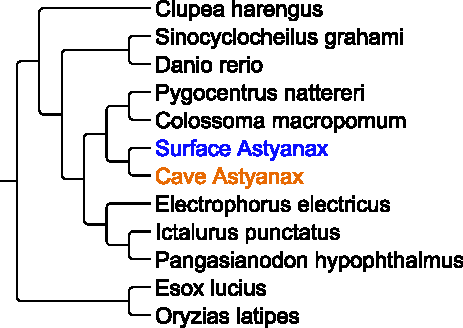
\includegraphics{Figures/astyanax/species_tree}
\caption[Species tree used for comparative genomics]{Species tree used for comparative genomics.}
\label{fig:methfig_species_tree}
\end{figure}

Once we provided all the necessary input for Progressive Cactus, the program started to align the different genomes in a referenceless manner. This process was the most computationally intense in this thesis since the process took one month to finish. Once the alignment was finished, the result was an alignment file in hal format. The Cactus toolkit allows the transformation of this hal file to a given set of alignment standard formats, giving a reference. We exported the alignments to MAF alignment files which can be read by downstream tools.

\subsection{Accelerated regions}

Once we produced the MAF files from the alignment, we started to use standard comparative genomics tools. One that has been key to understanding how \textit{Astyanax mexicanus} has adapted to the cave environment has been PHAST \parencite{hubisz_phast_2011}. Using these tools, we were able to compute regions that show an accelerated evolution ratio compared to other genomic regions. This analysis used several scripts, which can be found in GitHub under the folder \path{Comparative_genomics}. I strongly encourage the reader to check the vignettes in the \href{http://compgen.cshl.edu/phast/resources.php}{PHAST web page} in case he/she need to perform these analyses. We used the R interface for PHAST, the package rphast for these analyses. An R script can be found in the GitHub repository with the code that we used.

In the first place, we computed those intergenic regions that were conserved between all the species in the alignment except our species of interest. In our case, this translates to using all the genomes for this computation but the cavefish one. This is because we used these regions as a "baseline" for variation in our data. Hence, we could not use the species we tested for computing this baseline.

Once we computed the conserved regions, we calculated which regions were accelerated. In this step, we used the complete alignment with all the species. We kept those conserved regions that fulfil the following conditions:
\begin{enumerate}
    \item Regions have to be present in cavefish since it is our testing organism.
    \item Regions need to appear in at least five species.
    \item Regions need to be present in species that are close to cavefish. These species are Surfacefish, piranha, electric eel, and both catfish and tambaqui.
\end{enumerate}

Once we selected these candidate regions, we computed the acceleration rate in Cavefish, using the function phyloP from rphast package. The problem with this tool was that it does not compute statistical significance for the regions. We used an empirical approach to compute this P value, and that was done by using random alignments and comparing the distribution of acceleration in real data vs simulated random data. Once we did this, we selected those regions with a corrected $P value < 0.05$. The $P value$ was corrected using Benjamin-Hochberg. Finally, we wrote the resulting accelerated regions into a bed file.

Note that this analysis can be done for several species, as long as we compute conserved regions without the species of interest. We did this analysis not only for cavefish but also for the entire \textit{Astyanax mexicanus} species and for piranha. Once we obtained the BED file with accelerated regions, we performed several analyses with them. We crossed these regions with ATAC-seq peaks and perform the aforementioned analyses in the previous sections (\ref{meth:motif_enrichment}).